\begin{pastexam}[label={px:ccu-113-swa-03}]{中正資工所甲組 113 學年度 第 3 題}
（單選）

The following is an AVL tree, which is implemented/represented as an array. Please answer the following questions from Q1 to Q3.

\begin{center}
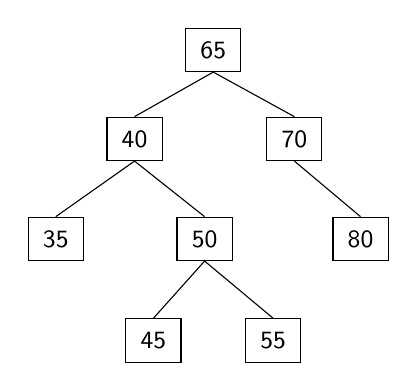
\begin{tikzpicture}[font=\sffamily\small]
\node[draw,rectangle,minimum width=7mm,minimum height=5.5mm,inner sep=1pt] (a) at (7.08,-5.92) {65};
\node[draw,rectangle,minimum width=7mm,minimum height=5.5mm,inner sep=1pt] (b) at (6.08,-7.05) {40};
\node[draw,rectangle,minimum width=7mm,minimum height=5.5mm,inner sep=1pt] (c) at (8.11,-7.05) {70};
\node[draw,rectangle,minimum width=7mm,minimum height=5.5mm,inner sep=1pt] (d) at (5.08,-8.32) {35};
\node[draw,rectangle,minimum width=7mm,minimum height=5.5mm,inner sep=1pt] (e) at (6.97,-8.32) {50};
\node[draw,rectangle,minimum width=7mm,minimum height=5.5mm,inner sep=1pt] (f) at (8.95,-8.32) {80};
\node[draw,rectangle,minimum width=7mm,minimum height=5.5mm,inner sep=1pt] (g) at (6.32,-9.61) {45};
\node[draw,rectangle,minimum width=7mm,minimum height=5.5mm,inner sep=1pt] (h) at (7.84,-9.61) {55};
\draw (a.south)--(b.north) (a.south)--(c.north) (b.south)--(d.north) (b.south)--(e.north) (c.south)--(f.north) (e.south)--(g.north) (e.south)--(h.north);
\end{tikzpicture}
\end{center}

(3\%) Remove the node with the key "65" from the AVL tree constructed for the first question (Q1) after the insertion. What does the array representation of the AVL tree look like?
\begin{enumerate}[label=\Alph*.]
\item (35, 45, 70, 40, 50, $-$, 80, $-$, 43, $-$, 55)
\item (55, 45, 70, 40, 50, $-$, 80, 43, 35)
\item (45, 40, 70, 35, 43, 50, 80, $-$, $-$, $-$, $-$, $-$, 55)
\item (45, 40, 70, 55, 43, 50, 80, 35)
\item None of the above
\end{enumerate}
\end{pastexam}

\begin{pastsoln}
答案是 C（以原卷的選項為準：C 的 $80$ 後面有五個 $-$，$55$ 在第 $13$ 格）。

照資結書第~10.2.6~節的刪除：要刪的節點有兩個子節點時，用\textbf{中序後繼}（右子樹的最小值）取代，再到右子樹刪掉
後繼；然後往上檢查平衡因子，遇到 $\pm 2$ 就旋轉。 起點是第 1 題插入 $43$ 之後的樹：
\[
65\Bigl(45\bigl(40(35, 43),\ 50(-, 55)\bigr),\ 70(-, 80)\Bigr).
\]

\textbf{刪除。} $65$ 有兩個子節點。 右子樹的最小值是 $70$（$70$ 沒有左子節點），用 $70$ 取代 $65$，再刪掉原來的
$70$ 節點，它只有右子節點 $80$，讓 $80$ 接上來。 得
\[
70\bigl(45(40(35, 43), 50(-, 55)),\ 80\bigr).
\]

\textbf{往上檢查。} 根 $70$ 的左子樹高 $3$、右子樹高 $1$，平衡因子 $+2$。 右邊少了一層，看左子節點 $B = 45$：它的左子樹
（$40$）高 $2$、右子樹（$50$）高 $2$，$\mathrm{BF}(B) = 0$，是 R0，對根做一次右旋（資結書第~10.2.6~節的表）：
$45$ 升為根，$45$ 原來的右子樹 $50(-, 55)$ 改掛到 $70$ 的左邊。
\[
45\Bigl(40(35, 43),\ 70\bigl(50(-, 55),\ 80\bigr)\Bigr).
\]
檢查：$40$ 是 $0$，$50$ 是 $-1$，$70$ 是 $+1$，根 $45$ 是 $2 - 3 = -1$，都平衡。
\begin{center}
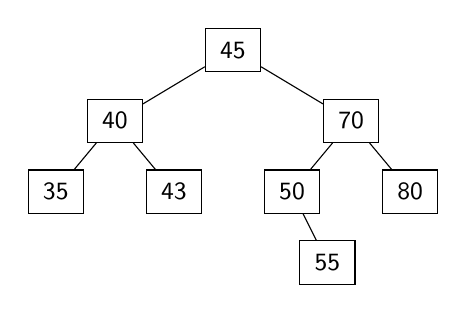
\begin{tikzpicture}[v/.style={draw,rectangle,minimum width=7mm,minimum height=5.5mm,inner sep=1pt,font=\sffamily\small},
  level distance=9mm, level 1/.style={sibling distance=30mm}, level 2/.style={sibling distance=15mm},
  level 3/.style={sibling distance=9mm}]
\node[v] {45}
  child {node[v] {40} child {node[v] {35}} child {node[v] {43}}}
  child {node[v] {70}
    child {node[v] {50} child[missing] child {node[v] {55}}}
    child {node[v] {80}}};
\end{tikzpicture}
\end{center}
陣列：第 $1$--$7$ 格是 $45, 40, 70, 35, 43, 50, 80$；$35, 43, 80$ 是葉子，第 $8$--$12$ 格都空；$55$ 是第 $6$ 格（$50$）的
右子節點，在第 $13$ 格：
\[
(45, 40, 70, 35, 43, 50, 80, -, -, -, -, -, 55),
\]
和原卷的 C 相同。

\textbf{如果用中序前驅。} 有些書刪除時改用左子樹的最大值（前驅）$55$ 取代 $65$。 刪掉原來的 $55$ 後 $50$ 變成葉子，
整棵樹 $55(45(40(35, 43), 50), 70(-, 80))$ 仍然平衡，陣列是 $(55, 45, 70, 40, 50, -, 80, 35, 43)$。 選項 B 是
$(55, 45, 70, 40, 50, -, 80, 43, 35)$，把 $35$、$43$ 左右放反了（$43 > 40$ 要在右邊），也不對。 所以兩種取代方法裡，
只有用後繼得到的 C 出現在選項中。

逐項檢查：
\begin{itemize}
\item A：根是 $35$，但 $35$ 是全樹最小值，左子樹必須是空的，卻放了 $45$。 錯。
\item B：見上，$35$ 放在 $40$ 的右邊，不是二元搜尋樹。 錯。
\item C：上面的結果。 對。
\item D：第 $4$ 格放 $55$，成了 $40$ 的左子節點，但 $55 > 40$。 錯。
\item E：C 是對的。 錯。
\end{itemize}
\end{pastsoln}
